%----------------------------------------------------------------------------------------
%	PACKAGES AND OTHER DOCUMENT CONFIGURATIONS
%----------------------------------------------------------------------------------------

\documentclass{article} % Paper and 12pt font size
\usepackage[utf8]{inputenc}
\usepackage[T1]{fontenc}
% \usepackage{libertine}
\usepackage{lmodern} % Use font Latin Modern Sans Typewriter
% \renewcommand{\familydefault}{\ttdefault}
\usepackage[a4paper, margin=1in]{geometry} % Paper size and margin

\usepackage{enumitem} % Format the enumerated list
\usepackage{amsmath,amsfonts,mathtools} % Math packages
\usepackage{amsthm}
\interdisplaylinepenalty=2500
\usepackage{amssymb}
\usepackage[makeroom]{cancel}
\setlength\parindent{0pt} % Removes all indentation from paragraphs - comment this line for an assignment with lots of text

\usepackage{array}
\usepackage{tabu} % Table to text width
\renewcommand{\arraystretch}{1.} % The height of each row in the table is set to 1.5 relative to its default height.
\usepackage[table]{xcolor}

\usepackage{tikz} % Remember picture
\usepackage{graphicx} % Includes images
\graphicspath{ {./images/} } % Tells LATEX that the images are kept in a folder named images under the directory of the main document
\usepackage{wrapfig} % Wrap image i
\usepackage{eso-pic} % used for image background on titlepage
\usepackage{subcaption} % subfigure

% Code listing style --------------
\usepackage{listings} % Code listing
\usepackage{color}
\definecolor{codegreen}{rgb}{0,0.6,0}
\definecolor{codegray}{rgb}{0.5,0.5,0.5}
\definecolor{codepurple}{rgb}{0.58,0,0.82}
\definecolor{backcolour}{rgb}{0.95,0.95,0.92}
\lstdefinestyle{mystyle}{
    backgroundcolor=\color{backcolour},
    commentstyle=\color{codegreen},
    basicstyle=\ttfamily\small,
    keywordstyle=\color{magenta},
    numberstyle=\tiny\color{codegray},
    stringstyle=\color{codepurple},
    breakatwhitespace=false,
    breaklines=true,
    captionpos=b,
    keepspaces=true,
    numbers=left,
    numbersep=5pt,
    showspaces=false,
    showstringspaces=false,
    showtabs=false,
    tabsize=2
}
\lstset{style=mystyle}
\usepackage{todonotes}  % Todo



%----------------------------------------------------------------------------------------
%	TITLE SECTION
%----------------------------------------------------------------------------------------
\title{\Huge \textbf{ASSIGNMENT 3} \vspace{.4in} \hrule}

\author{
	\Large ROB521: Mobile Robotics and Perception\\
	\Large Jojo (Yizhi) Zhou, 1003002396\\
}
\date{\normalsize\today}

\linespread{1.3}

\begin{document}
\fontfamily{lmtt} % modern typewriter font

%----------------------------------------------------------------------------------------
%	FRONT MATTER
%----------------------------------------------------------------------------------------
\begin{titlepage}
\tikz[remember picture,overlay]
\node[opacity=1] at (current page.center){
\includegraphics[width=\paperwidth,height=\paperheight]{../Background}};
\vspace*{3.5cm}
{\let\newpage\relax\maketitle}
\vspace*{\fill}

\end{titlepage}

% \newpage
\fontfamily{lmtt} % modern typewriter font

%----------------------------------------------------------------------------------------
%	Q1
%----------------------------------------------------------------------------------------
\section{Stereo Visual Odometry Results} % The * makes it an unnumbered section
In this project, we use stereo visual odometry to estimate the motion of a mobile robot, using a real image dataset. The resulting estimations are show below:

\begin{figure}[hbt]
  \centering
  \begin{subfigure}{.7\textwidth}
    \centering
    % include first image
    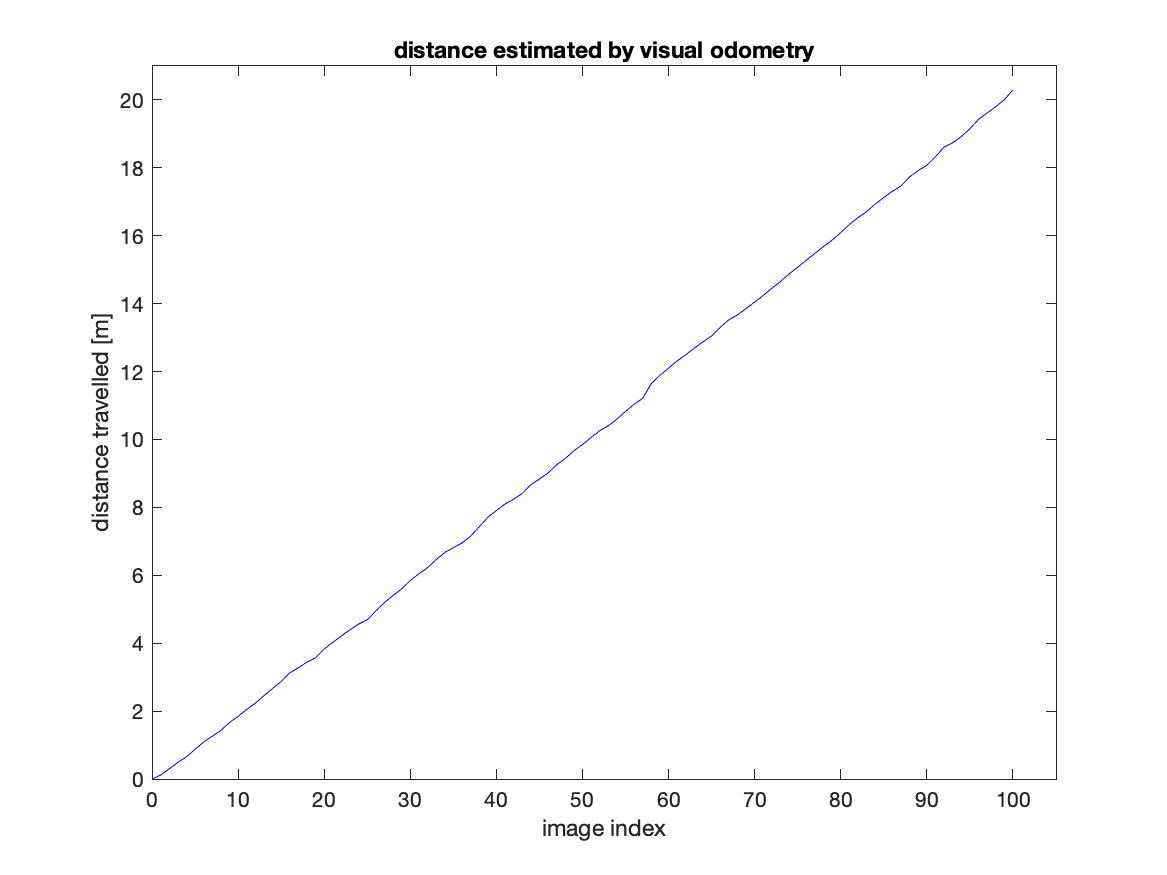
\includegraphics[width=1.\linewidth]{ass3_distance}
    \caption{Distance travelled.}
    \label{fig:sub-first}
  \end{subfigure}
  \begin{subfigure}{.7\textwidth}
    \centering
    % include second image
    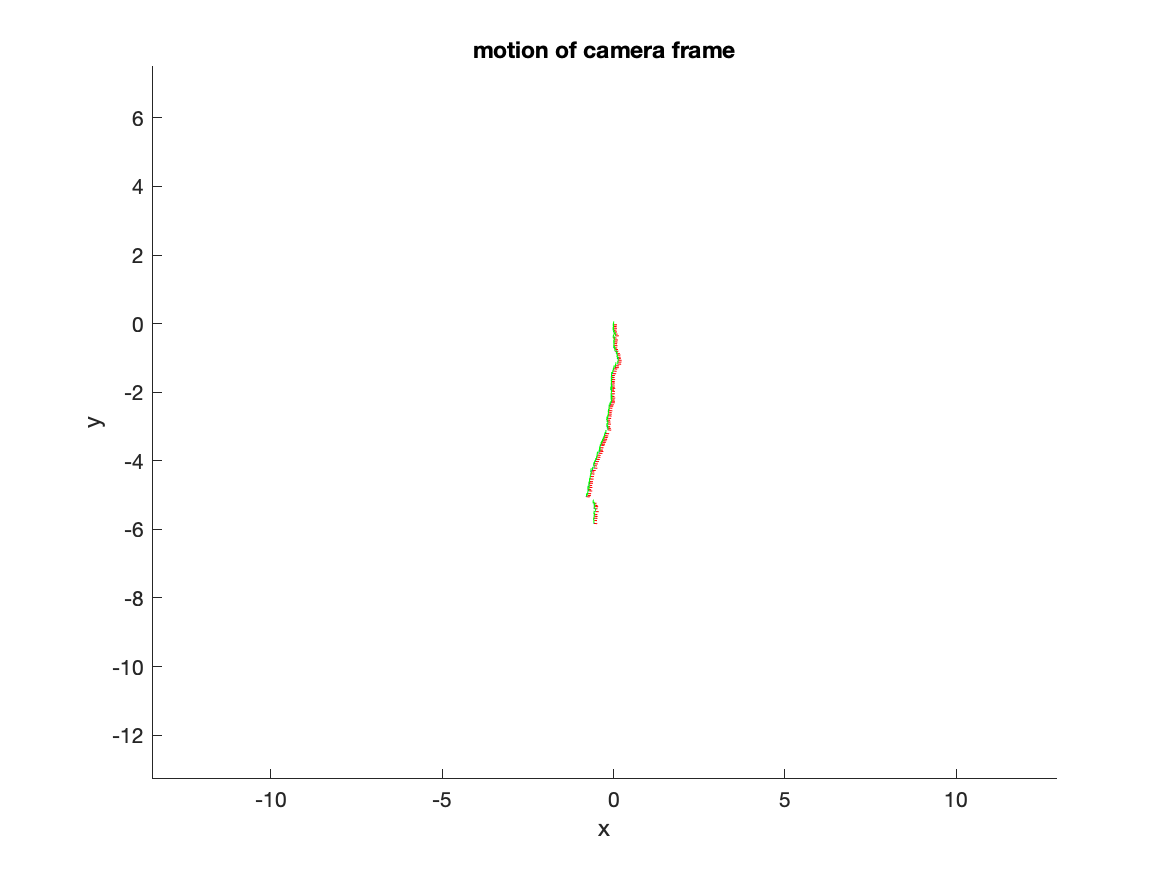
\includegraphics[width=1.\linewidth]{ass3_motion}
    \caption{Motion.}
    \label{fig:sub-second}
  \end{subfigure}
  \caption{Motion estimation with stereo visual odometry.}
\end{figure}

\clearpage
\section{Discussion} % The * makes it an unnumbered section
Figure \ref{fig:sub-first} shows the distance travelled by the robot, which linearly increases with time, indicating that the robot was likely traveling along a certain orientation at a constant speed. There are indeed some squiggles, probably as a result of the bumpy ground. However, the line has no discontinuity remains straight in general.

Figure \ref{fig:sub-second} shows the motion of camera frame and robot. There several aspects worth discussing:
\begin{itemize}
  \item The robot travels along $z$-direction in almost a straight path, which is very consistent to Figure \ref{fig:sub-first}.
  \item The blue and red represent the camera and robot, respectively. They are very close together and remains this way. This is also expected, as the camera and robot are supposed to be fixed together.
  \item There are a few discontinuities (e.g., at $z=2, 4, 8, 11$). They can be caused by the following
  \begin{itemize}
    \item RANSAC might have eliminated too many features in these frames that the matching was affected
    \item There could simply be no good feature at all in these frames - for example, when the robot is bumping through an obstacle, the camera could be shaking so much that the features are blurry or skewed.
  \end{itemize}
\end{itemize}

%----------------------------------------------------------------------------------------
%	Appendix
%----------------------------------------------------------------------------------------
\clearpage
\section*{Appendix: Source Code}
\lstinputlisting[language=matlab]{ass3.m}


\end{document}
